\documentclass[12pt,a4paper]{article}

% --- Packages essentiels ---
\usepackage[T1]{fontenc}
\usepackage[french]{babel}
\usepackage{amsmath, amssymb}
\usepackage{geometry}
\usepackage{graphicx}
\usepackage{tikz}
\usetikzlibrary{calc}
\usepackage{hyperref}
\usepackage{setspace}

\geometry{margin=1in}

% --- Hyperliens ---
\hypersetup{
    colorlinks=true,
    linkcolor=blue,
    urlcolor=blue,
    pdftitle={Postulat du Squaring},
    pdfauthor={Philippe Thomas Savard}
}

% Pas de numérotation sur la page titre
\pagenumbering{gobble}

\begin{document}



% --- Page titre ---
\begin{titlepage}
    \centering
    \vspace*{2cm}

    {\Huge \textbf{L'univers est au carré}}\\[0.5cm]
    {\Large \textbf{Chapitre : Le Postulat du Squaring}}\\[2cm]

    {\Large Auteur : \textbf{Philippe Thomas Savard}}\\[0.3cm]
    {\large Lévis, Chaudière-Appalaches, Canada}\\[0.3cm]
    {\large Treize mars deux mille vingt-six}\\[2cm]

    \vfill
\end{titlepage}

\clearpage
\pagenumbering{arabic}

\tableofcontents
\clearpage

% --- Message d'auteur ---
\begin{center}
\begin{minipage}{0.85\textwidth}
\small
\section*{Note de l’auteur}
\addcontentsline{toc}{section}{Note de l’auteur}

L’auteur de ce document n’a aucune formation académique reconnue. 
Il est ouvrier, et il a conçu ce travail sans financement, sans soutien institutionnel et sans aucun intérêt de quelque nature que ce soit. 
Ce document est rédigé et partagé librement, avec une pleine conscience et une lucidité entière.

Les sujets abordés relèvent des mathématiques et de la géométrie. 
Ils ont été explorés et développés par pur plaisir intellectuel, dans un esprit de curiosité, de rigueur personnelle et de liberté créative.
\end{minipage}
\end{center}

\vspace{1cm}

% --- Figure : Rectangle au carré ---
\begin{figure}[h!]
\centering
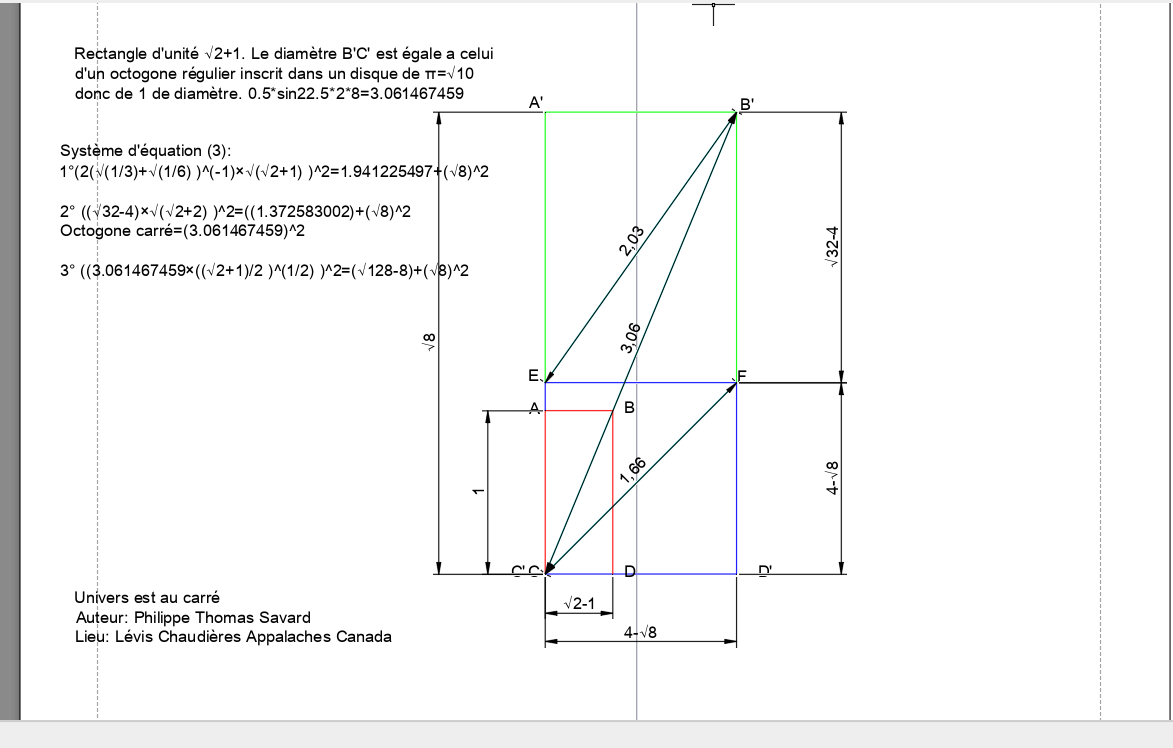
\includegraphics[width=0.85\textwidth]{racine_carre_deux.png}
\end{figure}



% --- Début du chapitre ---
\section{Explication mathématique du postulat du squaring}

\subsection{Le rectangle initial $ABCD$}

On considère un rectangle initial $ABCD$ tel que :
\[
AB = CD = \sqrt{2} - 1,
\qquad
AD = BC = 1.
\]

Son périmètre vaut :
\[
2(\sqrt{2}-1) + 2(1) = \sqrt{8}.
\]

\subsection{Élévation au carré : le rectangle $A'B'C'D'$}

En appliquant le postulat du squaring, on élève le périmètre au carré :
\[
(\sqrt{8})^2 = 8.
\]

Le rectangle transformé $A'B'C'D'$ possède alors :
\[
A'B' = C'D' = 4 - \sqrt{8},
\qquad
A'D' = B'C' = \sqrt{8}.
\]

Vérification :
\[
2(4-\sqrt{8}) + 2\sqrt{8} = 8.
\]

\subsection{Carré maximal inscrit dans $A'B'C'D'$}

Le plus grand carré inscrit dans $A'B'C'D'$ est $A'B'EF$.

Son aire vaut :
\[
(4-\sqrt{8})^2 = 1.372583002.
\]

L’aire du rectangle complet est :
\[
(4-\sqrt{8})\sqrt{8} = \sqrt{128} - 8.
\]

Le rapport des aires vaut :
\[
\frac{\sqrt{128}-8}{1.372583002} = \sqrt{2} + 1.
\]

Cette valeur devient l’unité symbolique de la mise en situation.

\subsection{Décomposition interne du rectangle transformé}

Le rectangle $A'B'C'D'$ contient :

\[
\text{Aire}(A'B'EF) = 1.372583002,
\qquad
\text{Aire}(EFC'D') = 1.941225497,
\]
\[
\text{Aire}(A'B'C'D') = \sqrt{128} - 8.
\]

On vérifie :
\[
(\sqrt{128}-8) = 1.372583002 + 1.941225497.
\]

Les dimensions des deux sous-figures sont :
\[
EF = 4 - \sqrt{8},
\qquad
C'D' = \sqrt{32} - 4.
\]

\subsection{Les trois diagonales fondamentales}

\[
\begin{aligned}
\text{Diag}(A'B'EF) &= \sqrt{32} - 4, \\
\text{Diag}(EFC'D') &= 2\left(\sqrt{\tfrac13} + \sqrt{\tfrac16}\right)^{-1}, \\
\text{Diag}(A'B'C'D') &= 3.061467459.
\end{aligned}
\]

La diagonale $A'C'$ est la mesure exacte du périmètre d’un octogone régulier inscrit dans un disque de diamètre $1$, donc :
\[
3.061467459 = \pi.
\]

Dans notre cadre géométrique :
\[
\sqrt{10} = \pi.
\]

\subsection{Les trois équations de l’octogone carré}

\[
\boxed{
\left( 2\left(\sqrt{\tfrac13}+\sqrt{\tfrac16}\right)^{-1} \sqrt{\sqrt{2}+1} \right)^2
= 1.941225497 + (\sqrt{8})^2
}
\]

\[
\boxed{
\left( (\sqrt{32}-4)\sqrt{\sqrt{2}+2} \right)^2
= 1.372583002 + (\sqrt{8})^2
}
\]

\[
\text{\small\itshape octogone carré}
\]

\[
\boxed{
\left( 3.061467459 \sqrt{\frac{\sqrt{2}+1}{2}} \right)^2
= (\sqrt{128}-8) + (\sqrt{8})^2
}
\]

\begin{figure}[h!]
\centering
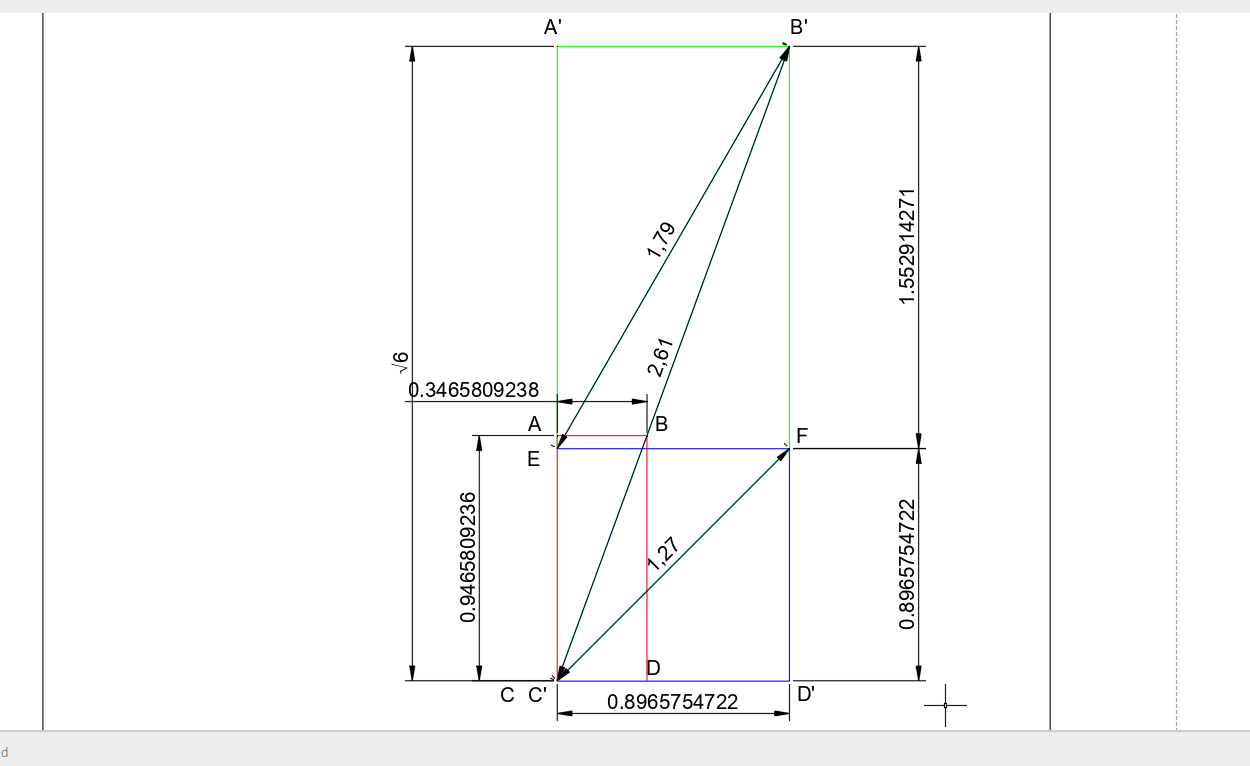
\includegraphics[width=0.85\textwidth]{racine_carre_trois.png}
\end{figure}
\setstretch{1.2}
% ---------------------------------------------------------
% SUITE DU TEXTE
% ---------------------------------------------------------

\section{Unité symbolique $\sqrt{3}+1$ : rectangle carré et hexagone carré}

\subsection*{Explication textuelle}

L’unité symbolique $\sqrt{3}+1$ donne naissance à une nouvelle famille géométrique, en parallèle à celle construite avec $\sqrt{2}+1$. Ici encore, on part d’un rectangle initial, on applique le postulat du \emph{squaring} au périmètre, puis on observe la structure interne du rectangle transformé. Cette fois, la figure mise en évidence n’est plus un octogone carré, mais un \emph{hexagone carré}.

On commence par un rectangle $ABCD$ dont les côtés sont choisis de sorte que son périmètre soit
\[
2AB + 2AD = 2.586915234.
\]
Ce périmètre est la racine carrée du périmètre d’un rectangle transformé $A'B'C'D'$, conformément au postulat du squaring. Le rectangle transformé a pour périmètre
\[
\sqrt{24} + 1.793150943 = 6.692130429.
\]
Ses côtés sont
\[
A'B' = 0.8965754715,
\qquad
A'D' = \sqrt{6},
\]
et il contient un segment horizontal $EF$ de même longueur que $A'B'$, situé à une hauteur
\[
B'F = 1.552914271.
\]

Comme dans le cas de l’unité $\sqrt{2}+1$, le rectangle transformé se décompose en deux régions : un rectangle carré $A'B'EF$ et un rectangle résiduel $EFC'D'$. Les aires et les diagonales de ces deux sous-figures, ainsi que celles du rectangle complet $A'B'C'D'$, permettent d’écrire trois équations remarquables. Ces équations mettent en relation l’unité $\sqrt{3}+1$, les longueurs internes de la figure et la diagonale du rectangle transformé.

La diagonale du rectangle transformé est liée au périmètre d’un hexagone régulier inscrit dans un disque de diamètre $1$, dont le périmètre vaut
\[
3.
\]
Ainsi, l’unité $\sqrt{3}+1$ joue pour l’hexagone un rôle analogue à celui que joue $\sqrt{2}+1$ pour l’octogone : elle encode une transformation géométrique où rectangle, carré et hexagone se répondent dans une même structure de squaring.

\subsection*{Développement en calculs}

\paragraph{Rectangle initial $ABCD$.}

On considère un rectangle initial $ABCD$ tel que :
\[
AB = 0.3465809239,
\qquad
AD = 0.9468766931.
\]
Son périmètre vaut :
\[
2(0.3465809239) + 2(0.9468766931)
= 2.586915234.
\]

\subsection{rectangle transformé}

En appliquant le postulat du squaring, le périmètre du rectangle transformé est :
\[
\sqrt{24} + 1.793150943 = 6.692130429.
\]

Le rectangle $A'B'C'D'$ possède :
\[
A'B' = 0.8965754715,
\qquad
A'D' = \sqrt{6},
\qquad
EF = 0.8965754715,
\qquad
B'F = 1.552914271.
\]

\[
\boxed{
\left( 1.793150943 \,\sqrt{\sqrt{3}+1} \right)^2
= 2(0.8965754715 \times 1.552914271) + (\sqrt{6})^2
}
\]

\[
\boxed{
\left( (3-\sqrt{3})\sqrt{\sqrt{3}+3} \right)^2
= 2(0.8038475761) + (\sqrt{6})^2
}
\]

\[
\text{\small\itshape hexagone carré}
\]

\[
\boxed{
\left( 2.608418597 \,\sqrt{\frac{2}{4-\sqrt{3}}\,\sqrt{3}} \right)^2
= 2(0.8965754715 \times \sqrt{6}) + (\sqrt{6})^2
}
\]

Enfin, le périmètre de l’hexagone régulier inscrit dans un disque de diamètre $1$ vaut :
\[
0.5 \times \sin(30^\circ) \times 2 \times 6 = 3.
\]

Ces trois équations définissent la figure élevée au carré associée à l’unité $\sqrt{3}+1$ :
\[
\text{l’hexagone carré}.
\]

\end{document}